\problem{Refract Facts}

\begin{wrapfigure}{r}{0.5\linewidth}
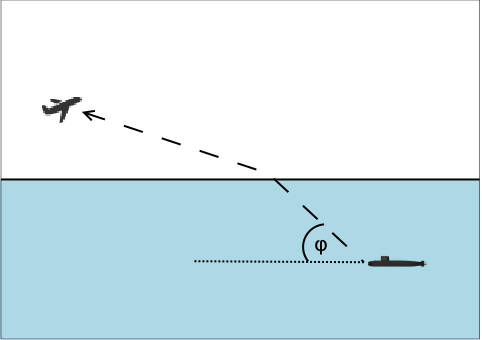
\includegraphics[width=\linewidth]{Refract/refract.png}
\end{wrapfigure}


A submarine is using a communications laser to send a message to a jet
cruising overhead.  The sea surface is flat. The submarine is cruising
at a depth $d$ below the surface. The jet is at height $h$ above the sea
surface, and a horizontal distance $x$ from the sub.  The submarine
turns toward the jet before starting communications, but needs to know
the angle of elevation, $\phi$, at which to aim the laser.

\begin{wrapfigure}{r}{0.5\linewidth}
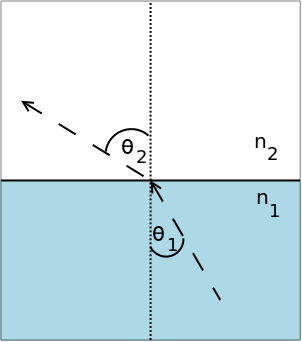
\includegraphics[width=\linewidth]{Refract/snell.png}
\end{wrapfigure}

When the laser passes from the sea into the air, it is refracted (its path is bent). The refraction is described by Snell's law, which says that light approaching the horizontal surface at an angle $\theta_1$, measured from the vertical, will leave at an angle $\theta_2$, given by the formula

\[ \frac{\sin \theta_1}{\sin \theta_2} = \frac{n_1}{n_2} \]

\noindent
where $n_1$ and $n_2$ are the respective {\em refraction indices} of
the water and air. (The refraction index of a material is inversely
proportional to how fast light can travel through that material.)

\subsection*{Input}

Input will consist of one or more datasets. 

Each dataset will consist of one line with 5 floating point
numbers. In order:

\begin{itemize}

\item $d$, the depth of the submarine (specifically, of the laser
  emitter) in feet, $1 \leq d \leq 800$

\item $h$, the height of the plane in feet, $100 \leq h \leq \num{10000}$

\item $x$, the horizontal distance from the sub to the plane in feet,
  $0 \leq x \leq \num{10000}$

\item $n_1$, the refractive index of water, $1.0 < n_1 \leq 2.5$, 

\item $n_2$, the refractive index of air, $1.0 \leq n_2 < n_1$ 
\end{itemize}

A value of 0 for $d$ will signal the end of input.

\subsection*{Output}

For each dataset, print a single line containing the angle of
elevation in degrees, to two decimals precision, at
which the submarine should aim its laser to illuminate the jet.




\subsection*{Example}

Given the input:

\verbfile{Refract/test0.in}


the output should be:

\verbfile{Refract/test0.expected}



